\documentclass[tikz,border=6pt]{standalone}
\usepackage{amsmath}
\definecolor{cA}{RGB}{31,94,165}\definecolor{cB}{RGB}{214,96,33}\definecolor{cC}{RGB}{46,139,87}
\tikzset{
  v/.style={circle,inner sep=0pt,minimum size=11pt,ball color=black!8,draw=black!55,line width=0.3pt},
  lab/.style={font=\small,fill=white,fill opacity=0.9,text opacity=1,inner sep=1.4pt,rounded corners=1pt},
  vl/.style={font=\footnotesize,inner sep=1pt},
  e2/.style={line width=1.6pt,cA!85},
  e3/.style={line width=1.6pt,cB!90},
  e5/.style={line width=1.6pt,cC!90}}
\pgfdeclarelayer{bg}\pgfsetlayers{bg,main}
\begin{document}
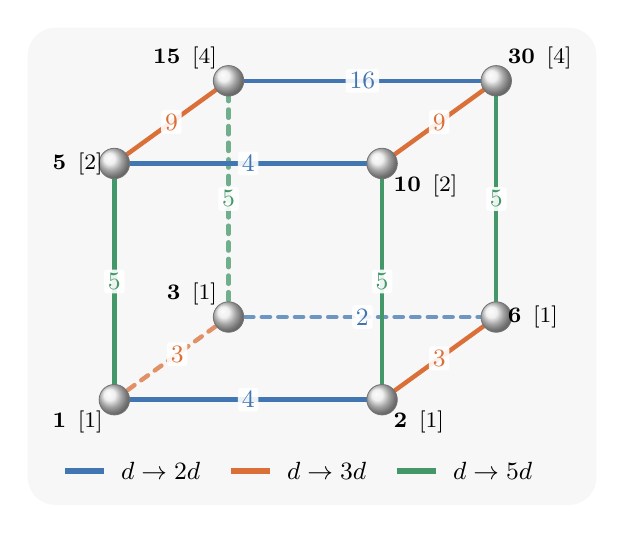
\begin{tikzpicture}[x={(3.4cm,0cm)},y={(1.45cm,1.05cm)},z={(0cm,3.0cm)},line cap=round]
% coordinates: (a,b,c) <-> 2^a 3^b 5^c ; x = factor 2, y = factor 3, z = factor 5
\coordinate (d1) at (0,0,0);  \coordinate (d2) at (1,0,0);
\coordinate (d3) at (0,1,0);  \coordinate (d6) at (1,1,0);
\coordinate (d5) at (0,0,1);  \coordinate (d10) at (1,0,1);
\coordinate (d15) at (0,1,1); \coordinate (d30) at (1,1,1);
% hidden edges first (behind)
\draw[e2,dashed,opacity=0.75] (d3) -- node[lab,pos=0.5] {$2$} (d6);
\draw[e3,dashed,opacity=0.75] (d1) -- node[lab,pos=0.55] {$3$} (d3);
\draw[e5,dashed,opacity=0.75] (d3) -- node[lab,pos=0.5] {$5$} (d15);
% visible edges
\draw[e2] (d1) -- node[lab] {$4$} (d2);
\draw[e2] (d5) -- node[lab] {$4$} (d10);
\draw[e2] (d15) -- node[lab] {$16$} (d30);
\draw[e3] (d2) -- node[lab] {$3$} (d6);
\draw[e3] (d5) -- node[lab] {$9$} (d15);
\draw[e3] (d10) -- node[lab] {$9$} (d30);
\draw[e5] (d1) -- node[lab] {$5$} (d5);
\draw[e5] (d2) -- node[lab] {$5$} (d10);
\draw[e5] (d6) -- node[lab] {$5$} (d30);
\foreach \d/\deg/\pos in {1/1/below left,2/1/below right,3/1/above left,6/1/right,5/2/left,10/2/below right,15/4/above left,30/4/above right}{
  \node[v] at (d\d) {};
  \node[vl,\pos=3pt] at (d\d) {$\mathbf{\d}\ \,[\deg]$};
}
% legend
\node[font=\small,anchor=west] at (-0.22,0,-0.30) {\color{cA!85}\rule[2pt]{14pt}{2pt}\ \ \color{black}$d\to2d$};
\node[font=\small,anchor=west] at (0.40,0,-0.30) {\color{cB!90}\rule[2pt]{14pt}{2pt}\ \ \color{black}$d\to3d$};
\node[font=\small,anchor=west] at (1.02,0,-0.30) {\color{cC!90}\rule[2pt]{14pt}{2pt}\ \ \color{black}$d\to5d$};
\begin{pgfonlayer}{bg}
\fill[black!3,rounded corners=10pt] ([shift={(-8pt,-6pt)}]current bounding box.south west) rectangle ([shift={(8pt,6pt)}]current bounding box.north east);
\end{pgfonlayer}
\end{tikzpicture}
\end{document}
